\documentclass[12pt,oneside,english,a4paper]{article}
\usepackage{babel}
\usepackage[utf8]{inputenc}
\usepackage[T1]{fontenc}
\usepackage{color}
\usepackage{graphicx}
\usepackage{wallpaper}
\usepackage{wrapfig,booktabs}

\usepackage{fancyhdr}

\usepackage{fourier-orns}
\newcommand{\dash}{\noindent \newline\textcolor{black}{\hrulefill~ \raisebox{-2.5pt}[10pt][10pt]{\leafright \decofourleft \decothreeleft  \aldineright \decotwo \floweroneleft \decoone   \floweroneright \decotwo \aldineleft\decothreeright \decofourright \leafleft} ~  \hrulefill}}

\usepackage{titlesec}
\titleformat*{\section}{\it\huge\bfseries}
\titleformat*{\subsection}{\it\huge\bfseries}
\titleformat*{\subsubsection}{\it\LARGE\bfseries}
\titleformat*{\paragraph}{\huge\bfseries}
\titleformat*{\subparagraph}{\LARGE\bfseries}

\usepackage[left=20px,right=20px,top=50px,bottom=50px,paperwidth=8in,paperheight=12in]{geometry}


\usepackage[cjk,usedotemph]{kotex}

\usepackage{amsthm} 
\usepackage{amsmath} 
\usepackage{amsfonts}
\usepackage{enumerate} 
\usepackage{cite}
\usepackage{graphics} 
\usepackage{graphicx,lscape} 
\usepackage{subcaption}
\usepackage{algpseudocode}
\usepackage{algorithm}
\usepackage{titlesec}
\usepackage{cite, url}
\usepackage{amssymb}

\def\bk{\paragraph{\LARGE$$}\LARGE}
\def\ck{\paragraph{\LARGE$\bullet$}\LARGE}
\def\pf{\paragraph{\LARGE(pf)}\LARGE}
\def\note{\paragraph{\LARGE\textit{\underline{note:}}}\LARGE}
\def\ex{\paragraph{\LARGE\textit{example:}}\LARGE}
\newcommand{\para}[1]{\paragraph{\LARGE\it\underline{\textbf{#1:}}}\LARGE}
\newcommand{\parablue}[1]{\paragraph{\LARGE\textcolor{blue}{\it\underline{\textbf{#1:}}}}\LARGE}
\newcommand{\parared}[1]{\paragraph{\LARGE\textcolor{red}{\it\underline{\textbf{#1:}}}}\LARGE}
\newcommand{\paraviolet}[1]{\paragraph{\LARGE\textcolor{violet}{\it\underline{\textbf{#1:}}}}\LARGE}
\newcommand{\paraorange}[1]{\paragraph{\LARGE\textcolor{orange}{\it\underline{\textbf{#1:}}}}\LARGE}


\def\one{\paragraph{\LARGE(1)}\LARGE}
\def\two{\paragraph{\LARGE(2)}\LARGE}
\def\three{\paragraph{\LARGE(3)}\LARGE}
\def\four{\paragraph{\LARGE(4)}\LARGE}
\def\five{\paragraph{\LARGE(5)}\LARGE}
\def\six{\paragraph{\LARGE(6)}\LARGE}
\def\seven{\paragraph{\LARGE(7)}\LARGE}
\def\eight{\paragraph{\LARGE(8)}\LARGE}
\def\nine{\paragraph{\LARGE(9)}\LARGE}
\def\ten{\paragraph{\LARGE(10)}\LARGE}

\def\cka{\paragraph{\LARGE(a)}\LARGE}
\def\ckb{\paragraph{\LARGE(b)}\LARGE}
\def\ckc{\paragraph{\LARGE(c)}\LARGE}
\def\ckd{\paragraph{\LARGE(d)}\LARGE}
\def\cke{\paragraph{\LARGE(e)}\LARGE}
\def\ckf{\paragraph{\LARGE(f)}\LARGE}
\def\ckg{\paragraph{\LARGE(g)}\LARGE}
\def\ckh{\paragraph{\LARGE(h)}\LARGE}
\def\cki{\paragraph{\LARGE(i)}\LARGE}
\def\ckj{\paragraph{\LARGE(j)}\LARGE}

\newcommand{\bs}[1]{\mbox{\boldmath $#1$}}

\newcommand{\bsa}{\mbox{\boldmath $a$}}
\newcommand{\bsb}{\mbox{\boldmath $b$}}
\newcommand{\bsc}{\mbox{\boldmath $c$}}
\newcommand{\bsd}{\mbox{\boldmath $d$}}
\newcommand{\bse}{\mbox{\boldmath $e$}}
\newcommand{\bsf}{\mbox{\boldmath $f$}}
\newcommand{\bsg}{\mbox{\boldmath $g$}}
\newcommand{\bsh}{\mbox{\boldmath $h$}}
\newcommand{\bsi}{\mbox{\boldmath $i$}}
\newcommand{\bsj}{\mbox{\boldmath $j$}}
\newcommand{\bsk}{\mbox{\boldmath $k$}}
\newcommand{\bsl}{\mbox{\boldmath $l$}}
\newcommand{\bsm}{\mbox{\boldmath $m$}}
\newcommand{\bsn}{\mbox{\boldmath $n$}}
\newcommand{\bso}{\mbox{\boldmath $o$}}
\newcommand{\bsp}{\mbox{\boldmath $p$}}
\newcommand{\bsq}{\mbox{\boldmath $q$}}
\newcommand{\bsr}{\mbox{\boldmath $r$}}
\newcommand{\bss}{\mbox{\boldmath $s$}}
\newcommand{\bst}{\mbox{\boldmath $t$}}
\newcommand{\bsu}{\mbox{\boldmath $u$}}
\newcommand{\bsv}{\mbox{\boldmath $v$}}
\newcommand{\bsw}{\mbox{\boldmath $w$}}
\newcommand{\bsx}{\mbox{\boldmath $x$}}
\newcommand{\bsy}{\mbox{\boldmath $y$}}
\newcommand{\bsz}{\mbox{\boldmath $z$}}

\newcommand{\bfa}{\mbox{$\bf{a}$}}
\newcommand{\bfb}{\mbox{$\bf{b}$}}
\newcommand{\bfc}{\mbox{$\bf{c}$}}
\newcommand{\bfd}{\mbox{$\bf{d}$}}
\newcommand{\bfe}{\mbox{$\bf{e}$}}
\newcommand{\bff}{\mbox{$\bf{f}$}}
\newcommand{\bfg}{\mbox{$\bf{g}$}}
\newcommand{\bfh}{\mbox{$\bf{h}$}}
\newcommand{\bfi}{\mbox{$\bf{i}$}}
\newcommand{\bfj}{\mbox{$\bf{j}$}}
\newcommand{\bfk}{\mbox{$\bf{k}$}}
\newcommand{\bfl}{\mbox{$\bf{l}$}}
\newcommand{\bfm}{\mbox{$\bf{m}$}}
\newcommand{\bfn}{\mbox{$\bf{n}$}}
\newcommand{\bfo}{\mbox{$\bf{o}$}}
\newcommand{\bfp}{\mbox{$\bf{p}$}}
\newcommand{\bfq}{\mbox{$\bf{q}$}}
\newcommand{\bfr}{\mbox{$\bf{r}$}}
\newcommand{\bfs}{\mbox{$\bf{s}$}}
\newcommand{\bft}{\mbox{$\bf{t}$}}
\newcommand{\bfu}{\mbox{$\bf{u}$}}
\newcommand{\bfv}{\mbox{$\bf{v}$}}
\newcommand{\bfw}{\mbox{$\bf{w}$}}
\newcommand{\bfx}{\mbox{$\bf{x}$}}
\newcommand{\bfy}{\mbox{$\bf{y}$}}
\newcommand{\bfz}{\mbox{$\bf{z}$}}

\newcommand{\bsA}{\mbox{\boldmath $A$}}
\newcommand{\bsB}{\mbox{\boldmath $B$}}
\newcommand{\bsC}{\mbox{\boldmath $C$}}
\newcommand{\bsD}{\mbox{\boldmath $D$}}
\newcommand{\bsE}{\mbox{\boldmath $E$}}
\newcommand{\bsF}{\mbox{\boldmath $F$}}
\newcommand{\bsG}{\mbox{\boldmath $G$}}
\newcommand{\bsH}{\mbox{\boldmath $H$}}
\newcommand{\bsI}{\mbox{\boldmath $I$}}
\newcommand{\bsJ}{\mbox{\boldmath $J$}}
\newcommand{\bsK}{\mbox{\boldmath $K$}}
\newcommand{\bsL}{\mbox{\boldmath $L$}}
\newcommand{\bsM}{\mbox{\boldmath $M$}}
\newcommand{\bsN}{\mbox{\boldmath $N$}}
\newcommand{\bsO}{\mbox{\boldmath $O$}}
\newcommand{\bsP}{\mbox{\boldmath $P$}}
\newcommand{\bsQ}{\mbox{\boldmath $Q$}}
\newcommand{\bsR}{\mbox{\boldmath $R$}}
\newcommand{\bsS}{\mbox{\boldmath $S$}}
\newcommand{\bsT}{\mbox{\boldmath $T$}}
\newcommand{\bsU}{\mbox{\boldmath $U$}}
\newcommand{\bsV}{\mbox{\boldmath $V$}}
\newcommand{\bsW}{\mbox{\boldmath $W$}}
\newcommand{\bsX}{\mbox{\boldmath $X$}}
\newcommand{\bsY}{\mbox{\boldmath $Y$}}
\newcommand{\bsZ}{\mbox{\boldmath $Z$}}

\newcommand{\bfA}{\mbox{$\bf{A}$}}
\newcommand{\bfB}{\mbox{$\bf{B}$}}
\newcommand{\bfC}{\mbox{$\bf{C}$}}
\newcommand{\bfD}{\mbox{$\bf{D}$}}
\newcommand{\bfE}{\mbox{$\bf{E}$}}
\newcommand{\bfF}{\mbox{$\bf{F}$}}
\newcommand{\bfG}{\mbox{$\bf{G}$}}
\newcommand{\bfH}{\mbox{$\bf{H}$}}
\newcommand{\bfI}{\mbox{$\bf{I}$}}
\newcommand{\bfJ}{\mbox{$\bf{J}$}}
\newcommand{\bfK}{\mbox{$\bf{K}$}}
\newcommand{\bfL}{\mbox{$\bf{L}$}}
\newcommand{\bfM}{\mbox{$\bf{M}$}}
\newcommand{\bfN}{\mbox{$\bf{N}$}}
\newcommand{\bfO}{\mbox{$\bf{O}$}}
\newcommand{\bfP}{\mbox{$\bf{P}$}}
\newcommand{\bfQ}{\mbox{$\bf{Q}$}}
\newcommand{\bfR}{\mbox{$\bf{R}$}}
\newcommand{\bfS}{\mbox{$\bf{S}$}}
\newcommand{\bfT}{\mbox{$\bf{T}$}}
\newcommand{\bfU}{\mbox{$\bf{U}$}}
\newcommand{\bfV}{\mbox{$\bf{V}$}}
\newcommand{\bfW}{\mbox{$\bf{W}$}}
\newcommand{\bfX}{\mbox{$\bf{X}$}}
\newcommand{\bfY}{\mbox{$\bf{Y}$}}
\newcommand{\bfZ}{\mbox{$\bf{Z}$}}

\DeclareMathOperator*{\argmin}{argmin} 
\DeclareMathOperator*{\argmax}{argmax} 
\renewcommand{\footnotesize}{\fontsize{9pt}{11pt}\Large}

\usepackage[svgnames]{xcolor}
\usepackage{listings}

\lstset{language=R,
    basicstyle=\LARGE\tt,
    stringstyle=\color{DarkGreen},
    otherkeywords={0,1,2,3,4,5,6,7,8,9},
    morekeywords={TRUE,FALSE},
    deletekeywords={data,frame,length,as,character},
    %keywordstyle=\color{blue},
    commentstyle=\color{DarkGreen},
}
\CJKscale{0.9}
\begin{document}
\section{Introduction}
\paraorange{본문} We consider the long-run behaviour of non-homogeneous Markov
chains, i.e. Markov chains in which the one-step transition probabilities are not constant. We are in effect concerned quite generally with infinite products of stochastic matrices. The number of states, $N$, will be assumed finite. The individual transition matrices will be denoted by $P_1,P_2,\dots,P_j\dots$ (The elements in all matrices are arranged so that the rows sum to $1$.) We define
\[
H_{i,n}=\prod_{j=i+1}^{i+n}P_j.
\]
Where convenient we shall write more simply
\[
H_n=H_{0,n}=\prod_{j=1}^{n}P_j.
\]
Let $H_{i,n}$ consist of elements $h_{\alpha,\beta}^{(i,n)}$. We define an \textcolor{blue}{\bf ergodic} chain as one for which, as $n\to \infty$,
\[
\big|h_{\alpha,\beta}^{(i,n)}-h_{\alpha',\beta}^{(i,n)} \big|\to 0 \quad \mbox{for any $i$ and all $\alpha$, $\alpha'$, $\beta$.} \quad \cdots (\ast)
\]
Condition (3) does not imply in general that the $h_{\alpha,\beta}^{(i,n)}$ themselves tend to a limit as $n \to \infty$. If such limits exist for all $\alpha,\beta$, and condition (3) is fulfilled, we shall say that \textcolor{blue}{\bf a chain is ergodic in the strong sense}. Chains which only fulfil ($\ast$) are \textcolor{blue}{\bf ergodic in the weak sense only}. When the term ergodic is used without qualification it covers all chains for which (3) is true.

\paraviolet{해설} (1) 이 논문에서는 넌-호모지니우스한 마코프체인의 롱-런 비헤이비어를 다룬다. 논의를 위하여 몇 가지 노테이션을 정의하자. $N$을 노드의 수로 정의하고 $P_1,P_2,P_3,\dots$을 각각 시점 1,2,3에서 전이확률이라고 하자. 이것을 활용하면 $i$시점에서 $n$시점의 전이확률을 아래와 같이 정의할 수 있다. 
\[
H_{i,n}=\prod_{j=i+1}^{i+n}P_j=P_{i+1}P_{i+2}\dots P_{i+n}
\]
이제 $H_{i,n}$의 $(\alpha,\beta)$-th 원소를 $h_{\alpha,\beta}^{(i,n)}$이라고 하자. 이는 $i$시점에서 $\alpha$노드에 있던 엔지니어가 그로부터 $n$시점 이후에\footnote{그러니까 $i+n$시점에서} $\beta$노드에 있을 확률을 의미한다. (2) 에르고딕 체인이라고 함은 모든 $i$와 모든 노드 $\alpha,\alpha',\beta$에 대하여 아래가 성립하는 마코프체인을 의미한다. 
\[
\big|h_{\alpha,\beta}^{(i,n)}-h_{\alpha',\beta}^{(i,n)} \big|\to 0 \quad \mbox{for any $i$ and all $\alpha$, $\alpha'$, $\beta$.} \quad \cdots(\ast)
\]
그러니까 $n\to \infty$라면 초기에 엔지니어가 $\alpha$회사에서 근무했던 $\alpha'$회사에서 근무했던 결국 회사 $\beta$에서 근무하고 있을 확률이 동일하다는 의미이다. (3) 중요한 부분은 약 에르고{\bf 디}시티와 강 에르고{\bf 디}시티를 구분이다. 저자들은 ($\ast$)를 만족하면 약 에르고{\bf 디}시티를 만족하는 조건이지만 이것이 강 에르고{\bf 디}시티는 아니라는 점을 분명히 하였다. 또한 약 에르고{\bf 디}시티는 $h_{\alpha,\beta}^{(i,n)}$자체가 극한을 가지는 것이 아니라는 것을 분명히 하였다. 이는 트랜지션-매트릭스가 진동하지만 정상상태로 가는 경우를 생각하면 이해하기 쉽다. 트랜지션-매트릭스 $P$의 각 원소가 수렴하지 않지만 특정한 2개의 값으로 진동한다고 하자. 예를들어 노드 $\alpha$에서 노드 $\beta$로 갈 확률이 0과 1의 값으로 진동한다고 하면 $P$자체는 극한을 가지지 않지만 무한걸음이후에 엔지니어가 노드 $\beta$에서 근무할 확률은 수렴한다. 

\paraorange{본문} This paper is a development of an earlier paper [Hajnalm, 1956] devoted mainly to strong ergodicity. The definition of ergodicity given above is, however, slightly more restricted
than that in the earlier paper, which required only that $H_{0,n}$ tend to a matrix with {\bf identical rows}. The restriction that such a tendency must hold for $H_{i,n}$ in starting at any
trial $i$, means that cases where the differences between rows of $H_{0,n}$ disappear only because of a finite number of the $P_j$ are not classed as ergodic. The following cases can occur:
\begin{enumerate}[(i)]
	\item A finite number of the $P_j$ may themselves be matrices with identical rows.
	\item $H_{0,n}$ may be a matrix with identical rows for some finite $n$. This can happen even if none of the $P_j$ has identical rows, e.g. let 
	\[
	P_1=\begin{bmatrix}
	\frac{1}{3} & \frac{2}{9} & \frac{4}{9} \\
	\frac{1}{3} & 0 & \frac{2}{3} \\
	\frac{1}{3} & \frac{1}{3} & \frac{1}{3} 
	\end{bmatrix},\quad 
	P_2=\begin{bmatrix}
	1 & 0 & 0 \\
	\frac{1}{3} & \frac{1}{3} & \frac{1}{3} \\
	\frac{1}{3} & \frac{1}{3} & \frac{1}{3} 
	\end{bmatrix}.
	\]
	Then 
	\[
	H_2=\begin{bmatrix}
	\frac{5}{9} & \frac{2}{9} & \frac{2}{9} \\
	\frac{5}{9} & \frac{2}{9} & \frac{2}{9} \\
	\frac{5}{9} & \frac{2}{9} & \frac{2}{9} 
	\end{bmatrix}.
	\]
	\item Let $P_1$ be the same as in (ii) and let 
	\[
	H_{1,n}=\begin{bmatrix}
	1 & 0 & 0 \\
	\frac{1}{3} & \frac{1}{3} & \frac{1}{3} \\
	\frac{1}{3} & \frac{1}{3} & \frac{1}{3} 
	\end{bmatrix} \quad\mbox{as } n\to\infty.
	\]
	Then $H_{0,n}$ tends to a matrix with identical rows, but not $H_{1,n}$, $H_{2,n}$
\end{enumerate}

\paraviolet{해설} (1) [Hajnal,1956]이전에 연구되었던 다른 페이퍼들은 강 에르고{\bf 디}시티를 아래의 조건을 만족하는 체인으로 정의하였다. 
\[
H_{0,n}\to \mbox{matrix with identical rows}
\]
위에서 matrix with identical rows를 줄여서 \textcolor{blue}{\bf MwIR}이라고 하자. 그런데 이 조건은 합리적이지 않다. 위의 조건이 $i$에 상관없이 성립하면 좋겠다. 왜냐하면 (i)-(iii)의 경우가 가능하기 때문이다. (i)의 경우는 유한개의 $P_j$만 MwIR인 경우이고 (ii)의 경우는 $P_j$가 모두 MwIR은 아니지만 $H_2=H_{0,2}=P_1P_2$가 MwIR이 되는 경우이고 (iii)은 $H_{0,n}$이 MwIR로 수렴하지만, $H_{1,n}$과 $H_{2,n}$은 MwIR로 수렴하지 않는 경우를 의미한다. (그래서 멀 어쩌라는거임)

\paraorange{본문} The proposed definition is not only essential for much of the mathematics that follows, but also seems required from the point of view of applications.\footnote{먼가 새로운 정의를 제안하는데 이게 수학적으로 중요하다기 보다 다양한 어플리케이션에 적용가능하다는 이야기인듯?} An ergodic chain, as here defined, has the property that knowledge of its state at \emph{any} trial is of no avail\footnote{어{\bf베}이ㄹ, 도움이 되다} for forecasting the state in which it will be in the distant\footnote{먼,멀리떨어진} future. In other words, an ergodic chain is one which `forgets' the distant past (and not only the initial state). Another aspect appears in Theorem 4. 
\bk Homogeneous chains, if they are ergodic at all, are ergodic in the strong sense. In this case special tools become available and these have generally been used for deriving the ergodic properties of homogeneous chains. Thus the general problem of ergodicity has largely escaped attention.

\paraviolet{해설} (2) 일단 호모지니우스한 마코프체인에서는 에르고딕하면 무조건 강에르고딕이다. 

\section{A special class of matrices}

\paraorange{본문} Ergodic homogeneous chains are usually termed
\textcolor{blue}{\bf regular}. Chains can be non-regular if (i) there are two or more groups of states between which transitions are not possible, or (ii) there are two or more groups of states such that transition is possible only between groups and not within them. Chains under (i) are \textcolor{blue}{\bf decomposable}, those under (ii) \textcolor{blue}{\bf periodic}. This classification of homogeneous chains amounts to a classification of stochastic matrices $P$ by the behaviour of $P_n$ as $n\to \infty$.
\bk To which of these classes a matrix belongs, is determined only by the number and position of the non-zero elements in it. This will be termed the pattern of a matrix. It is important to note that: (a) the product of two non-regular matrices may be regular and (b) the products of regular matrices may not be regular. The following patterns
(where $\times$ denotes a non-zero element) illustrate these facts:
\begin{figure}[h]
\center
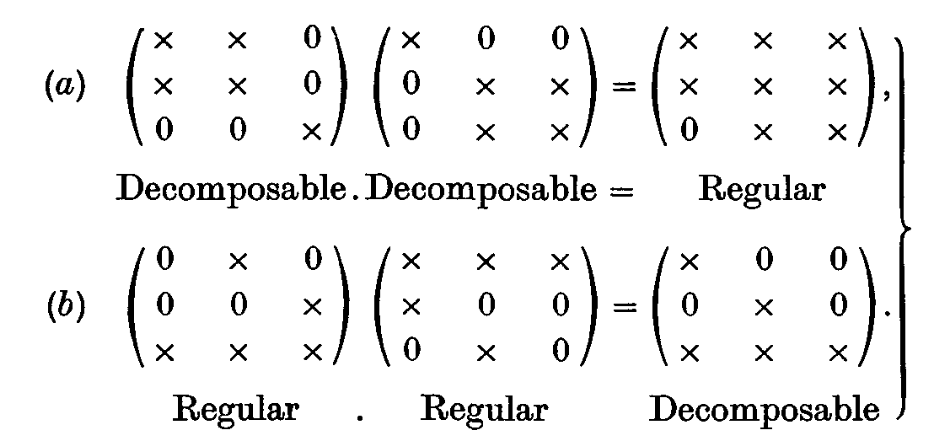
\includegraphics[width=1\textwidth]{Fig1.png}
\caption{논문에 있는 그림}
\end{figure}
\bk Phenomenon (b) shows that little can be expected from methods using characteristic roots. Regular matrices have only a single characteristic root of unit modulus. Decomposable matrices have more than one root equal to unity. Hence, as example (b) shows, the roots of a product of two stochastic matrices may be of larger modulus
than the roots of the factors. In the homogeneous regular case the moduli of all except one of the characteristic roots of
\[
H_n=P^n
\]
decrease as $n$ increases, and it is this fact which is used to investigate the ergodic properties. 

\paraviolet{해설} {\bf (1)} 호모지니우스-마코프체인이 에르고딕하면 그 전이확률 $P$를 \textcolor{blue}{\bf 레귤러}하다고 표현한다. 레귤러하지 않은 $P$는 크게 \textcolor{blue}{\bf 분해가능행렬(decomposable matrix)}인 경우와 \textcolor{blue}{\bf 주기행렬(periodic)}인 경우로 나눌 수 있다.\footnote{[Hajnal,1956]에 따르면 레귤러하지 않은 경우는 2가지 경우 뿐이 없는것 같다. 그리고 [Hajnal,1956]에 따르면 레귤러 매트릭스의 경우 항상 {\bf limit}을 가지며 그 limit은 항상 모든 row가 동일한 매트릭스가 나온다.} (i) 먼저 $P$가 분해가능행렬인 경우를 살펴보자. 이는 두개 혹은 그 이상의 회사간에 이동이 불가능한 경우를 의미한다.\footnote{엔지니어들이 갈수 있는 회사계열이 크게 사기업계열과 공기업계열로 나누어진다고 하자. 사기업에 한번 취업한 엔지니어는 공기업계열로 절대 이직불가능하다는 룰이 있다면 이러한 체인을 분해가능하다고 표현한다.} (ii) 다음은 $P$가 주기행렬인 경우를 살펴보자. 이는 노드들이 몇개의 그룹으로 나누어지고 그룹간의 이동만 가능한 형태이다.\footnote{엔지니어들이 갈수있는 회사계열은 크게 사기업계열과 공기업계열로 나누어진다고 하자. 만약에 사기업계열에서 1년일하면 반드시 그 이후에는 공기업계열에서 일을 해야한다는 룰이 있다면 이러한 체인을 피리오딕하다고 표현한다.} 이러한 매트릭스들\footnote{분해가능, 주기}은 매트릭스에서 어떤 위치에 $0$이 존재하는지에 따라 결정된다.\footnote{당연한거 아닌가?} {\bf (2)} 그런데 흥미로운 점은 (a) 넌레귤러한 매트릭스의 곱이 레귤러 할수도 있고 (b) 레귤러매트릭스의 곱이 레귤러하지 않을 수도 있다는 것이다. 여기에서 (b)가 의미하는 바가 중요한데 (b)는 $P$의 고유치를 이용해서 뭔가를 분석하는 방법\footnote{methods using characteristic roots}이 한계가 있음을 보여준다. 

\paraorange{본문} 
It may be inferred from the above examples that ergodic chains may consist entirely of non-regular matrices arranged in suitable sequence. Similarly, non-ergodic chains may consist entirely of regular matrices. 

\bk We shall therefore define a special subclass of regular matrices, having the following properties:
\begin{enumerate}[(i)]
	\item A product of which one factor belongs to this class, will itself belong to this class.
	\item The occurrence of an infinite sequence of matrices of this class will (subject to certain natural conditions) ensure that the chain is ergodic.
\end{enumerate}
\bk The following classes suggest themselves as having the required properties. There is, first, the class of matrices with no zero elements. (A theorem on weak ergodicity using this class was given in the earlier paper [Hajnalm, 1956].) A second more extended class is that of matrices with at least one column, all of whose elements are non-zero.
\paraviolet{해설}

\paraorange{본문(scrambling matrix)} The most extensive class of this kind is defined by the following characteristic. \textcolor{blue}{Given any two rows, say $\alpha$ and $\beta$, there exists at least one column, $\gamma$, such that both $p_{\alpha, \gamma} > 0$ and $p_{\beta,\gamma}>0$.} A matrix of this class will be called a \textcolor{blue}{\bf scrambling matrix}\footnote{스크{\bf 램}블링, 뒤죽박죽.}
\bk The idea of this class arises from the consideration that an ergodic chain is one which forgets its past. Suppose that after a trial subject to a scrambling matrix $P$ we find the system in state $\gamma$. Then we cannot be sure whether it was in state $\alpha$ or in state $\beta$ before the trial. A scrambling matrix is one in which the probabilities of transition from different initial states are not all in distinct columns, but as it were, scrambled.

\paraviolet{해설} (1) 견우와 직녀가 각각 마코프이직을 한다고 하자. 어떠한 이직 시점 $\ell$에 대해서 견우와 직녀가 각각 일하는 회사를 서로 $\alpha$ $\beta$라고 하자. $(\alpha,\beta)$의 조합에 관계없이 견우와 직녀는 $\ell+1$시점에서 최소한 하나의 회사\footnote{가칭 $\gamma$회사, 약속의 회사..}에서 같이 일할 희망이 있다고 하자. 그러면 이러한 마코프이직을 스크{\bf 램}블링 하다고 한다. (2) 과거를 추적할 수 없는 $\gamma$가 하나라도 존재하면 스크{\bf 램}블링 마코프이직이다.\footnote{결국에는 이 미꾸라지 같은 $\gamma$때문에 모든 체인의 과거이력이 점점 꼬이기 시작한다. 이러한 내용이 레마 1,2,3에 증명되어 있다.} 

\paraorange{본문} For the subsequent\footnote{{\bf 섭}시컨트, 그 다음의, 차후의} argument a measure of the `scrambling power' of a matrix $P$
is needed, i.e. of the degree to which it approaches a matrix with identical rows which scrambles all traces of the past. Let the measure be denoted by $\{P\}$. We first form for each pair of rows $\alpha$, $\alpha'$ the sum $\sum_{\beta}\min(p_{\alpha,\beta},p_{\alpha',\beta})$. $\{P\}$ is defined as the smallest of these sums, i.e.
\[
\{P\}=\min_{\alpha,\alpha'}\sum_{\beta}\min(p_{\alpha,\beta},p_{\alpha',\beta}).
\]
It will easily be seen that:
\begin{enumerate}[(i)]
\item $\{P\}$ lies between $0$ and $1$; 
\item $\{P\}=0$ if and only if $P$ is not a scrambling matrix;
\item $\{P\}=1$ if and only if all rows of $P$ are identical.
\end{enumerate}

\paraviolet{해설} 이 패러그랩에서 이해할 것은 크게 2개가 있다. (1) 첫번째는 스크램블링 매트릭스의 개념을 잡는 것이다. 스크램블드된 정도는 $\{P\}$로 측정할 수 있다. $\{P\}=0$이면 스크{\bf 램}블드 되어 있지 않다는 의미이다.\footnote{즉 모든 과거를 추적가능 할 수 있다는 것임. 대표적으로 $\tt node1 \to node2 \to node3 \to node1$형태의 마코프이직.} $\{P\}=1$은 극도로 스크램블드 되어있다는 의미이다. 아래의 느낌을 기억하면 편리하다. 
\begin{itemize}
	\item {\bf erogodicity:} 스크램블드, MwIR, 레귤러, 정상분포를 가짐
	\item {\bf non erogodicity:} not 스크램블드, 이레귤러, 피리오딕 or {\bf 디}콤{\bf퍼}저블
\end{itemize}
(2) 두번째로 이해할것은 저자들이 도대체 왜 $\{P\}$라는 것을 왜 정의할까? 라는 점이다. 생각해보자. 극도로 스크램블드된 경우, 즉 $\{P\}=1$인 경우는 MwIR이다. 그런데 앞으로 논문의 진행방향은 $H_{0,n} \to \mbox{MwIR}$와 같이 강한 조건을 
\[
H_{0,n} \to P, \quad \mbox{with } \{P\}\approx 1
\]
와 같이 약한 조건으로 바꾼뒤 에르고{\bf 디}시티를 조사하고 싶을 것이다. 그리고 이를 위해서는 $\{P\}$의 정의가 필수적이다. (3) 이제 $\{P\}=\min_{\alpha,\alpha'}\sum_{\beta}\min(p_{\alpha,\beta},p_{\alpha',\beta})$를 계산하는 방법에 대하여 알아보자. 아래의 과정을 따른다. 
\begin{enumerate}[(i)]
\item 제일 비슷해보이는 임의의 2개의 row를 고른다. 골라진 노드의 인덱스를 각각 $(\alpha,\alpha')$ 라고 둔다. 
\item 골라진 2개의 로우의 원소를 서로 column-wisely 비교해가면서 2개중의 작은 값만 골라서 더한다. 그리고 이값을 $\{P\}$라고 둔다. 
\end{enumerate}
다시 한번 살펴보자. $P$는 스토캐스틱 매트릭스이므로 선택된 $\alpha$-th row의 모든 원소합은 1이다. 마찬가지의 논리로 선택된 $\alpha'$-th row의 모든 원소합은 1이다. 하지만 2개의 로우를 서로 column-wisely 비교해가면서 2개중의 작은 값만 골라서 더한다면 어떨까? 두 rows가 완전히 같지 않은 이상, 항상 이 값은 1보다 작을 것이다. 바로 이 값이 바로 $\{P\}$라는 소리이다. 
(4) 따라서 잘 생각해보면 결국 동일한 rows가 한쌍이라도 있으면 $\{P\}=1$이 된다는 것을 알 수 있다. 따라서 $\{P\}=1$은 MwIR보다 훨씬 약한 조건이다. 따라서 스크램블링 매트릭스는 MwIR보다 훨씬 훨씬 더 약한 조건이다. 

\paraorange{본문} The following lemmas show how the scrambling property is preserved in a chain whatever other transition matrices may follow after a scrambling matrix.
\para{Lemma 1} If $L$ and $M$ are stochastic matrices and $Q=LM$, then $\{Q\} \geq \{L\}.$


\para{Lemma 2} If $L$ and $M$ are stochastic matrices and either of them is a scrambling matrix, so is $Q=LM$.

\paraviolet{해설} 기본적으로 $L$은 before $M$은 transition $Q$는 after를 의미한다. 따라서 레마2가 의미하는건 before / transirion 중 하나라도 스크램블되어 있으면, after도 스크램블된다는 것을 의미한다.\footnote{즉 $H_{0,n}$의 limit이 스크{\bf 램}블링 매트릭스가 아닐려면, 초기분포와 모든 전이행렬이 스크램링 매트릭스가 아닌경우밖에 없다. 즉 어지간하면 스크램블드 매트릭스란 소리다.} 또한 레마1이 의미하는건 스크램블되는 정도가 점점 심해진다는 것을 의미한다. 즉 레마 1,2는 결국 시간이 지날수록 에르고드한 성질이 점점 강해진다는 것을 의미한다. 

\paraorange{본문} An important property which distinguishes scrambling matrices is stated in the following theorem.

\para{Theorem 1} Let $X$ be a stochastic matrix. There exists another stochastic matrix $Y$ such that $Z=XY$ is a non-regular matrix, if and only if $X$ is not a scambling matrix.

\paraviolet{해설} $X$가 스크램블링 매트릭스가 아님을 주장하려면 어떻게 해야하는가? 정리1에 의하면 $X$에 적당한 매트릭스 $Y$를 곱해서 넌-레귤러 매트릭스를 만들면 된다. 즉 $X$를 적당히 선형변형시켜\footnote{즉 $Y$를 곱해서} (1) 분해가능 행렬을 만들거나 (2) 주기행렬을 만들어 내면 된다는 것이다. 

\section{Conditions for weak ergodidty}
\paraorange{본문} To study ergodic chains we need to measure not
only the scrambling power of the individual transition matrix $P_j$ but also the accumulated scrambling effect on
\[
H_n=\prod_{j=1}^{n}P_j
\]
$\{H_n\}$ may be used for the latter purpose also; but if this is done, the argument becomes laborious. It is easier to introduce a second measure, as follows:
For any matrix $A$ with elements $a_{\alpha,\beta}$ we define 
\[
[A]=\max_{\beta}\max_{\alpha,\alpha'}|a_{\alpha,\beta}-a_{\alpha',\beta}|.
\]
Thus $[A]$, which may be called the maximum range of $A$, is the maximum difference between any pair of elements in the same column.
$[H_n]$ is zero if and only if all rows of $H_n$ are identical, i.e. $[H_n]$ is roughly analogous to $1-\{H_n\}$. However, whereas $1-\{H_n\}$ can only decrease as $n$ increase, $[H_n]$ can both increase and decrease. 

\paraviolet{해설} (1) $H_n$이 스크램블된 정도를 특정하는 또 다른 메져 $[H_n]$을 만들자. $[H_n]$은 $H_n$의 row들간의 차이를 메져한다. 따라서 대략 $[H_n]\approx 1-\{H_n\}$의 느낌이다. 하지만 완전히 $[H_n]=1-\{H_n\}$인 것은 아니다. $[H_n]$과 $1-\{H_n\}$의 공통점과 차이점은 무엇일까? 공통점은 모두 MwIR을 기준으로 삼는다는 점이다. 즉 $H_n$이 MwIR일때 $[H_n]=0$이고 $1-\{H_n\}=0$이다. 차이점은 $1-\{H_n\}$은 항상 $n$이 커짐에 따라 감소하기만 하지만, $[H_n]$은 증가하기도 하고 감소하기도 한다. (2) $[P]$를 구하는 방법은 아래와 같다. 
\begin{enumerate}[(i)]
\item 원소들의 min,max가 가장 극단적인 column $\beta$를 찾는다. 
\item column $\beta$의 range를 구한다. 이 값이 $[P]$이다. 
\end{enumerate}
(3) $P$가 MwIR의 경우 $P$의 어떠한 컬럼 $\beta$를 fix해도 칼럼들의 원소는 모두 같은 값이다.\footnote{이 값이 의미하는 것은 다른 임의의 노드에서 $\beta$노드로 이직할 확률을 의미한다. 즉 이 값이 0.2라는 것은 엔지니어가 지금 어떤 회사에서 근무하든지 다음에 $\beta$회사에서 근무할 확률이 0.2이라는 의미이다.} 따라서 이 경우에 $[P]=0$이다. 

\paraorange{본문} We first prove 

\para{Lemma 3} If $F=PG$ where $P$ and $G$ are stochastic matrices, then 
\[
[F] \leq (1-\{P\})[G].
\]

\paraviolet{해설} (1) $F$는 after, $P$는 before, $G$는 transition을 의미한다. 따라서 위의 식은
\[
\mbox{F의 non-ergodicity} \leq \mbox{P의 non-ergodicity} \times \mbox{G의 non-ergodicity}
\]
의 느낌인데 양변에 $f(x)=1-x$를 취하면 
\[
\mbox{F의 ergodicity} \geq \mbox{P의 ergodicity} \times \mbox{G의 ergodicity}
\]
의 느낌으로 해석할 수도 있다. 즉 레마3도 레마1,2의 연장선상에 있는데 시간이 지날수록 에르고드한 성질이 점점 강해진다는 것을 의미한다. (2) 레마3의 또 다른 의미는 바로 $[A]$와 $\{A\}$의 관계를 알려준다는 것이다. 예를들면 아래의 {\bf 코}럴래러리와 같은 결과를 알게 해준다. 

\paraorange{본문} By applying Lemma 3 to the product $AI$, where $I$ is the identity matrix, we obtain
\para{Corollary} $[A] \leq (1-\{A\})$.

\paraviolet{해설} 생략.

\paraorange{Theorem 2} For any Markov chain 
\[
[H_n] \leq \prod_{j=1}^{n-1}(1-\{P_j\})[P_n] \leq \prod_{j=1}^{n}(1-\{P_j\}).
\]
\bk Theorem 2 gives an upper bound for the differences between rows of $H_n$. As applied to regular homogeneous chain with transition matrix $P$ this result shows that the difference between $h_{\alpha,\beta}^{(n)}$ and its limit (as $n\to \infty$) is less than $(1-\{P\})^n$. A better estimate can often be obtained by taking, with some suitable $k$, 
\[
(1-\{P^k\})^{n/k}.
\]
If $P$ is a regular but not a scrambling matrix, it is in any case necessary to take $k$ large enough to make $P_k$ a scrambling matrix, if a useful estimate is to be obtained. Estimates obtained from Theorem 2 are at least as good as, and generally better than, those obtainable by earlier methods.


\paraviolet{해설} 결국 위의 {\bf 코}러레어리는 정리2로 확장할 수 있다. 정리2는 difference between rows of $H_n$의 upper bound에 대한 이야기를 한다. 그러니까 예를들어 이런식으로 쓸 수 있다. (1) 만약에 $P$가 레귤러 호모지니우스한 체인의 전이확률이라고 하자. 그러면 정리2에 의해서
\[
\left|h_{\alpha,\beta}^{(n)}-\lim_{n\to\infty} h_{\alpha,\beta}^{(n)}\right| \leq (1-\{P\})^n
\]
가 성립한다.(왜?\footnote{레귤러 호모지니우스하므로 $P^n$은 MwIR로 수렴한다는 사실을 이용하면 좌변이 이해된다.}) (2) 따라서 아래와 같은 식도 성립함도 쉽게 알 수 있다. 
\[
\left|h_{\alpha,\beta}^{(n)}-\lim_{n\to\infty} h_{\alpha,\beta}^{(n)}\right| \leq (1-\{P^k\})^{n/k}
\]
이는 $P$가 레귤러이지만 스크램블링 매트릭스는 아닐 경우\footnote{이런경우가 있나?}, 그런데 적당히 큰 $k$를 취해서 스크램블링 매트릭스를 만들수는 있는 경우 유용하다. 

\paraorange{본문} These earlier methods can also be applied to non-homogeneous chains, and it may be convenient to do so since $\{P_j\}$ is often laborious\footnote{러{\bf 보}리우스, 힘든} to compute. For example, if we denote by $\{P_j\}^\ast$ the sum of the smallest elements in each column of $P_j$, we have
\[
\{P_j\}^\ast \leq \{P_j\}.
\]
Hence we may add a 
\para{Corollary to Theorem 2} For any Markov chain 
\[
[H_n]\leq \prod_{j=1}^{n-1}(1-\{P_j\}^\ast)[P_n]\leq \prod_{j=1}^{n}(1-\{P_j\}^\ast).
\]
An even rougher estimate of $[H_n]$ is obtained by putting in place of $\{P_j\}$ simply the smallest element in any one column. 

\paraviolet{해설} 종종 $\{P_j\}$를 계산하는 것이 너무 러{\bf 보}리우스 하면 $\{P_j^\ast\}\leq \{P_j\}$를 만족하는 적당한 $\{P_j\}^\ast$를 구해서 정리2에 대한 {\bf 코}럴래러리를 위와 같이 만들어서 쓰면 된다. 이게 무슨말인지 알아보자. $\{P_j\}$를 계산하기 위해서는 각 컬럼에서 비슷해보이는 임의의 2개의 row를 선택해야한다. 그리고 선택된 row들을 columwise비교하여 작은 값을 더해버린다. 그런데 이렇게 2개의 row를 선택하기 귀찮다면, 모든 row에 대하여 columwise하게 비교해가면서 작은값을 더한뒤 이를 $\{P_j\}^\ast$라고 한뒤,\footnote{자동으로 $\{P_j\}^\ast \leq \{P_j\}$가 성립한다.} 위의 {\bf 코}럴래러리를 쓰면 된다는 것이다. 

\paraorange{본문} Theorem 2 leads to a condition for ergodicity. We may cover ergodic chains where the sequence of $P_j$ includes no infinite subsequence of scrambling matrices by applying Theorem 3 to blocks of successive transition matrices. 

\para{Theorem 3} A Markov chain is ergodic if and only if there exists a subdivision of the sequence of trials into blocks at trials numbered $i_1,i_2,i_3,\dots$, such that $\sum_{j=1}^{\infty}\{H_{i_j,n_j}\}$ diverges.
Here $n_j=i_{j+1}-i_j$; i.e. $H_{i_j,n_j}$ is the matrix of probabilities that the system pass from being in state $\alpha$ after trial $i_j$ to being in state $\beta$ after trial $i_{j+1}$.

\paraviolet{해설} 걸음을 적당한 간격으로 나누자. 예를들어서 아래와 같이 나눈다. 
\[
[\textcolor{red}{1},2,3],[\textcolor{red}{4},5],[\textcolor{red}{6},7,8,9,10],[\textcolor{red}{11}],[\textcolor{red}{12},13],\dots
\]
$i_1,i_2,i_3,\dots$는 각각 위에서 붉은색으로 표시된 인덱스이다. 즉 
\[
(i_1,i_2,i_3,i_4,i_5,\dots)=(1,4,6,11,12,\dots)
\]
이다. $n_1=\mbox{"첫번째 블락의 원소수"}$이다. 따라서 
\[
(n_1,n_2,n_3,n_4,n_5,\dots)=(3,2,5,1,2,\dots)
\]
이다. 대응하는 전이확률을 나열하면 
\[
[P_1,P_2,P_3],[P_4,P_5],[P_6,P_7,P_8,P_9,P_{10}],[P_{11}],[P_{12},P_{13}],\dots
\]
블락별로 전이확률을 곱하자. 즉 
\begin{align*}
H_{i_1,n_1}&=H_{1,3}=P_1P_2P_3 \\
H_{i_2,n_2}&=H_{4,2}=P_4P_5 \\
H_{i_3,n_3}&=H_{6,5}=P_6P_7P_8P_9P_{10} \\
H_{i_4,n_4}&=H_{11,1}=P_{11} \\
H_{i_5,n_5}&=H_{12,2}=P_{12}P_{13} 
\end{align*}
만약에 우리가 
\[
\{H_{i_1,n_1}\}+\{H_{i_2,n_2}\}+\{H_{i_3,n_3}\}+\dots = \infty
\]
임을 주장할 수 있다면 이 체인은 약 에르고드한 체인임을 주장할 수 있고 역도 성립한다. 


\paraorange{Corollary to Theorem 3} A Markov chain for which $\sum \{P_j\}$ diverges is ergodic. 

\paraviolet{해설} 당연한소리를. 

\paraorange{본문} We use now Theorem 3 to demonstrate an interesting special characteristic of ergodic chains. Consider two systems independently undergoing trials governed by
the same chain. We shall say that the systems are apart if they are in different states; if they are in the same state after a trial they will be said to meet at that trial (one may envisage two particles simultaneously performing the same random walk).

\paraviolet{해설} 생략 

\paraorange{Theorem 4} For ergodic chains, and for such chains only, the probability is one that if the two systems are ever apart they will meet at least once (and, therefore, infinitely often).

\para{Proof}
\paraviolet{해설} 정리4는 증명도 읽어 볼만한듯. 

\paraorange{본문} We now apply Theorem 3 to some chains whose sequence of transition matrices contains no infinite subsequence of scrambling matrices. In order to do this, restrictions must be placed on the patterns of the transition matrices. The word pattern refers, as before, to an arrangement of non-zero elements in a matrix. We shall speak of the pattern of a matrix, i.e. the arrangement of all non-zero elements in it. More generally we shall refer to the various patterns contained in a matrix, i.e. the pattern of the matrix and also all other patterns which may be formed from it by substituting zeros for one or more non-zero elements. Any theorem stating that chains having transition matrices of certain patterns are ergodic, clearly applies to all chains whose transition matrices contain those patterns.

\paraviolet{해설} 생략 

\paraorange{본문} The patterns of two matrices will be said to \textcolor{blue}{\bf commute} if the pattern of the product is the same in whichever order they are multiplied, while the value of the elements in
the product will, of course, in general depend on the order of multiplication. We first prove

\para{Lemma 4} A Markov chain is ergodic if 
\begin{enumerate}[(i)]
	\item each transition matrix contains the same regular pattern, and 
	\item the elements in this pattern in each matrix are greater than $\delta>0$.
\end{enumerate}

\paraorange{Theorem 5} A Markov chain is ergodic if each transition matrix contains a pattern such that the following three conditions are fulfilled: 
\begin{enumerate}[(i)]
\item all patterns commute with one another; 
\item regular patterns occur at intervals of at most $a$ matrices (where $a$ is any finite integer); 
\item all elements in the patterns are greater than $\delta>0$.
\end{enumerate}

\paraorange{Corollary} A Markov chains is ergodic if 
\begin{enumerate}[(i)]
	\item all transition matrices have regular commuting patterns; 
	\item all elements in the patterns are greater than $\delta>0$. 
\end{enumerate}

\section{An approximation theorem} 

\paraorange{본문} The discussion in section 2,3 may be very roughly summarized by saying that if the transition matrices $P_j$ of a chain have sufficiently large elements (in suitable positions) the chain will be ergodic.\footnote{$P_j$가 각각 충분한 수의 원소를 가지면, 즉 다음턴에 어디로 이직할지 모르게 만들면 에르고딕이다.} We can approach the problem from the other side. Starting from a non-ergodic chain  we may consider other chains which differ from it only in that the transition matrices have been very slightly modified. How small must these modifications be to ensure that the modified chain will, like the original chain, not be ergodic? The previous paper [Hajnal, 1956] discussed this problem for the special class of chains with commutative transition matrices. It was shown, for example, that there exist chains whose $j$th transition matrices $P_j$ (though none of them have any zero elements) tend, as $j\to\infty$, so rapidly to the identity matrix that the chain is not ergodic. 
\bk This phenomenon suggests the following general problem: how closely must the transition matrices of two chains be alike to ensure that they will have the same long-run behaviour? An answer to this question is provided by Theorem 6. 
We classify types of long-run behaviour as shown in the table below in accordance with the discussion in section 1 above. 
\begin{figure}[h]
\center
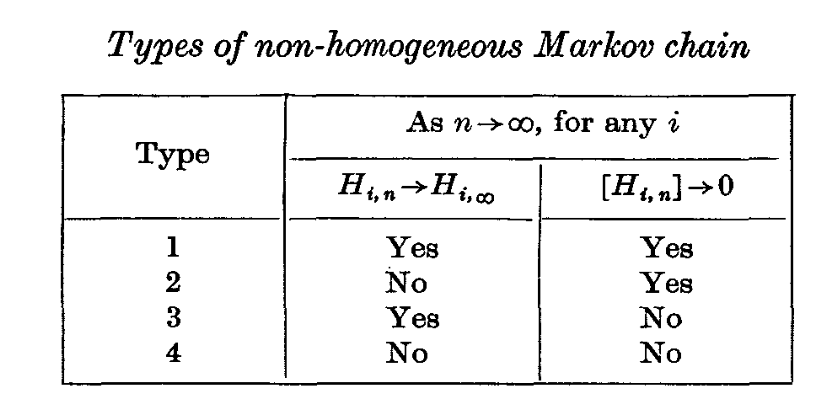
\includegraphics[width=1\textwidth]{Fig2.png}
\caption{논문에 있는 표: In the terminology here used types 1 and 2 are ergodic (type 1 in the strong sense, type 2 in the weak sense only). Types 3 and 4 are not ergodic.}
\end{figure}
For types 3 and 4 we have by definition that $[H_{i_0,n}]>\delta>0$ for some $i_0$ and an infinite subsequence of values of $n$. However, we may make a more general statement since it follows that $[H_{i,n}]\geq \delta/N$ for all $i>i_0$ and all $n$. For let $n_0$ be such that $[H_{i_0,n_0}]>\delta$ and suppose that $i_0<i'<i_0+n_0$ and $n'<i_0+n_0-i'$. We may write by Theorem 3 
\[
[H_{i_0,n_0}]\leq (1-\{H_{i_0,i'-i_0}\})(1-\{H_{i',n'}\})(1-\{H_{i'+n',i_0+n_0-n'-i'}\}).
\]
All factors have modulus less than 1, hence each must be greater than $\delta$. In particular 
\[
(1-\{H_{i',n'}\})>\delta.
\]
Hence by equation $N[P]\geq (1-\{P\})$\footnote{논문의 식 (20)에 있는 수식임, 여기에서 $N$은 노드의 총수를 의미함.}, 
\[
[H_{i',n'}]\geq \delta/N.
\]
As a preliminary\footnote{프리-{\bf 리}미내어리} to Theorem 6 we prove a lemma about infinite products of stochastic matrices. (Similar propositions are easily seen to hold for other suitably restricted types of matrix products.) 

Consider two chains. Let the $j$th transition matrix of the first chain be $P_j$ and of the second 
\[
\bar{P}_j=P_j+E_j.
\]
Let $e_j$ be the modulus of the element of largest modulus in $E_j$ and let $H_{i,n}=\prod_{j=i+1}^{i+n}P_j$ and $\bar{H}_{i,n}=\prod_{j=i+1}^{i+n}\bar{P}_j$.

\para{Lemma 5} If $\sum e_j$ converges, then for any $\epsilon$, there exists $i_0(\epsilon)$ such that for all $i>i_0$ and all $n$ 
\[
\left|(\bar{H}_{i,n}-H_{i,n}) \right|<\epsilon.
\]
\para{Remark} For any matrix $A$, $|A|$ denotes the modulus of the element of largest modulus in $A$. 

\bk To state Theorem 6 consider as before two chains and denote by $e_j$ the modulus of the largest difference between corresponding elements in the $j$th transition matrix. 

\paraorange{Theorem 6} If $\sum e_j$ converges, the two chains have the same type of long-run behaviour. 

\section{Strong ergodicity} 

\paraorange{본문} The more general conditions for weak ergodicity developed above may be usded to extend the conditions for strong ergodicity given in [Hajnal, 1956]. In effect a non-homogeneous chain is strongly ergodic if (a) it is weakly ergodic (by whatever means this may be proved), and (b) certain other conditions are fulfilled. For example, we may restate Theorem 1 of the previous paper in the following form. 
\para{Theorem 7} A weakly ergodic Markov chain for which there exists a sequence of stochastic matrices $S_1,S_2\dots$ with identical rows such that 
\begin{enumerate}[(i)]
\item $\sum|S_jP_{j+1}-S_{j+1}|$ converges. 
\item and $S_j\to S$, as $j\to\infty$.
\end{enumerate}
is ergodic in the strong sense and the limiting matrix is $S$. Other Theorems in the earlier paper can be similarly\footnote{{\bf시}밀래(를)리} generalized. 
\end{document}

 